\documentclass{assignment}

\usepackage{float}
% \usepackage{tikz}
\usepackage{circuitikz}
\usepackage{adjustbox}
\usepackage{titlesec}
\usepackage{soul}
\usepackage{csvsimple}

\usepackage{graphicx}
\usepackage{subcaption}
\usetikzlibrary{shapes, arrows}

\usetikzlibrary{calc,patterns,angles,quotes}
\setlength{\parindent}{0pt}

\hypersetup{
pdftitle={Lab - Mechatronics},
pdfsubject={Report for the MagLev laboratory experience},
pdfauthor={Tommaso Bocchietti, Daniele Cianca, Sara Orazzo},
pdfkeywords={Politecnico di Milano, Mechatronics, Magnetic Levitation System}
}

\makenoidxglossaries
\newacronym{mls}{MLS}{Magnetic Levitation System}
\newacronym{siso}{SISO}{Single Input Single Output}
\newacronym{miso}{MISO}{Multiple Input Single Output}
\newacronym{mimo}{MIMO}{Multiple Input Multiple Output}
\newacronym{pid}{PID}{Proportional Integral Derivative}
\newacronym{mpc}{MPC}{Model Predictive Control}
\newacronym{lqr}{LQR}{Linear Quadratic Regulator}

\begin{document}

\title{Lab - Mechatronics \\ Modelling and control of a Magnetic Levitation System}
\author{Tommaso Bocchietti 10740309 \\ Daniele Cianca 10764733 \\ Sara Orazzo 10995845}
\date{A.Y. 2024/25}

\maketitle

\begin{figure}[H]
    \centering
    \includegraphics[width=0.7\textwidth]{./pdf/Polimi_logo_coverpage.pdf}
    \label{fig:Polimi_logo}
\end{figure}

\clearpage
\tableofcontents
\listoffigures
\listoftables
% \lstlistoflistings
% \printnoidxglossaries

\clearpage
\section{Introduction}

\begin{frame}{Magnetic Levitation System (MLS)}

    Magnetic Levitation System (MLS) is an electromechanical system that enhances magnetic fields to levitate a ferromagnetic object.
    It's known for its non-linear behavior and its instability.

    \begin{figure}[H]
        \centering
        \includegraphics[width=0.5\textwidth]{./img/Maglev_from_the_lab.jpeg}
        \caption{Magnetic Levitation System used in this work.}
    \end{figure}

    The variable magnetic field is generated by two electromagnets driven in voltage, while the position of the ball is measured by an optical infrared sensor.

\end{frame}



\begin{frame}{Project objectives}

    \vspace{9pt}

    \begin{columns}[c, onlytextwidth]

        \begin{column}{0.5\textwidth}

            \begin{figure}[H]
                \centering
                \includegraphics[width=0.8\textwidth]{./img/ball_levitation.jpeg}
                \caption{Sphere levitating}
            \end{figure}

        \end{column}

        \begin{column}{0.5\textwidth}

            \begin{center}
                Project objectives: \\
                \textbf{Make the ball levitate.}
            \end{center}

        \end{column}

    \end{columns}

\end{frame}




\clearpage
\section{Magnetic Levitation System}
\label{sec:magnetic_levitation_system}

As stated in the introduction, the system under study is the \acrfull{mls} provided by \texttt{Inteco} (producer website: \url{https://www.inteco.com.pl/products/magnetic-levitation-systems/}).
In Figure \ref{fig:MLS} the system used in this work is shown.

\begin{figure}[H]
    \centering
    \includegraphics[width=0.7\textwidth]{./img/maglev_and_components.jpg}
    \caption{\acrlong{mls}}
    \label{fig:MLS}
\end{figure}

As it can be seen quite clearly, the system is composed of a simple mechanical structure that is used to support two electromagnets and an optical infrared sensor.
Along with the mechanical structure, a ferromagnetic ball and a control unit are present.

At its core principle, the system uses the interaction between the magnetic field generated by the electromagnets and the ferromagnetic ball to keep the ball in a desired position.
The optical sensor is used to measure the position of the ball and provide feedback to the control unit that, in turn, adjusts the voltage applied to (and indeed the current flowing through) the electromagnets to keep the ball in a desired position.
In Figure \ref{fig:MLS_general_scheme} a schematic representation of the upper half of the system is shown.

\begin{figure}[H]
    \centering
    \includegraphics[width=0.9\textwidth]{./img/maglev_general_scheme.png}
    \caption{Schematic representation of the upper half of the \acrshort{mls} system.}
    \label{fig:MLS_general_scheme}
\end{figure}

\paragraph{Real world application}

Despite the fact that our system is a simplified use case, the magnetic levitation principle is used in many real-world applications.

One of the most common applications is the magnetic levitation trains, also known as `MagLev' trains.
These trains use the magnetic levitation principle to lift the train off the tracks and propel it forward using the magnetic field generated by the tracks.
The main advantage of this technology is the absence of friction between the train and the tracks, which allows the train to reach higher speeds and reduce the noise characteristic of the traditional trains.
Some of the fastest (operating) trains in the world are MagLev trains, with the Shanghai MagLev train being the fastest, reaching a top speed of $623 km/h$ \cite{WikiSCMaglev}.

Another application of the magnetic levitation principle is the magnetic bearings.
These bearings use the magnetic field generated by electromagnets to levitate a rotor and keep it in a desired position.
The main advantage of this technology is the absence of mechanical contact between the rotor and the stator, which allows the rotor to reach higher speeds and reduce the wear of the components.

\clearpage
\section{Modelling}
\label{sec:modelling}

The \acrshort{mls} is a complex system that can be divided into:

\begin{itemize}
    \item \textbf{Electromagnetic subsystem}: it takes into account all the electrical components going from the power supply to the electromagnets themselves, and so the generation of the magnetic field by the coils;
    \item \textbf{Mechanical subsystem}: it takes into account the dynamics of the ball and the forces acting on it, including the electromagnetic forces generated by the magnetic field.
\end{itemize}

Due to the presence of the ball that moves inside a magnetic field, a complex connection between the two subsystems that goes beyond the simple force balance exists.
For this reason, it's almost impossible to derive a complete model without considering both subsystems at the same time.

In Figure \ref{fig:system_model}, a schematic representation of all the components of the system and the forces acting on it is shown.
Instead, in Table \ref{tab:components} a brief description of the components is provided.

\begin{figure}[H]

    \begin{minipage}{0.40\textwidth}

        \centering

        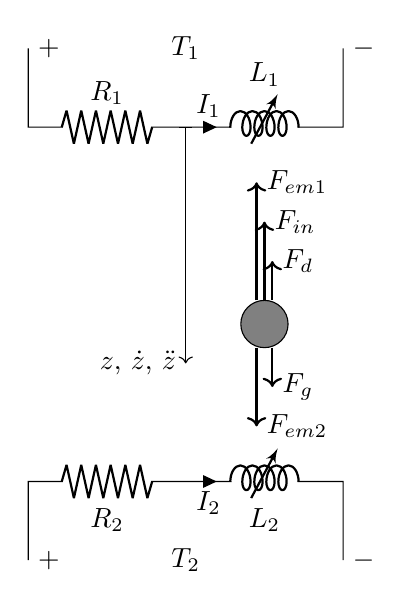
\begin{tikzpicture}[european voltages]

            \def\radius{0.3}

            % Upper circuit
            \node at (-1.0, 3.5) {$T_1$};
            \draw (-3, 3.5) node [right] {$+$}
            to [short] ++(0, -1)
            to [R, l^=$R_1$, resistors/zigs=6] ++(2, 0)
            to [variable cute inductor, i>^=$I_1$, l=$L_1$] ++(2, 0)
            to [short] ++(0, +1) node [right] {$-$};

            % Reference system
            \draw[|->] (-1.0, +2.5) -- ++(0, -3) node[left] {$z$, $\dot{z}$, $\ddot{z}$};

            % Ball
            \filldraw[fill=gray, draw=black] (0, 0) circle (\radius);

            % Upward forces
            \draw[thick, ->] (-0.1, +\radius) -- ++(0, +1.5) node[right] {$F_{\text{em1}}$};
            \draw[thick, ->] (+0.0, +\radius) -- ++(0, +1.0) node[right] {$F_{\text{in}}$};
            \draw[thick, ->] (+0.1, +\radius) -- ++(0, +0.5) node[right] {$F_{\text{d}}$};

            % Downward forces
            \draw[thick, ->] (+0.1, -\radius) -- ++(0, -0.5) node[right] {$F_{\text{g}}$};
            \draw[thick, ->] (-0.1, -\radius) -- ++(0, -1.0) node[right] {$F_{\text{em2}}$};

            % Lower circuit
            \node at (-1.0, -3.0) {$T_2$};
            \draw (-3, -3) node [right] {$+$}
            to [short] ++(0, +1)
            to [R, l_=$R_2$, resistors/zigs=6] ++(2, 0)
            to [variable cute inductor, i>_=$I_2$, l_=$L_2$] ++(2, 0)
            to [short] ++(0, -1) node [right] {$-$};

        \end{tikzpicture}

    \end{minipage}
    %
    \hfill
    %
    \begin{minipage}{0.55\textwidth}

        \centering

        \begin{tabular}{|c|l|c|}
            \hline
            \textbf{Name}      & \textbf{Description}               & \textbf{Units} \\
            \hline
            $F_{\text{g}}$     & Gravitational force                & N              \\
            $F_{\text{in}}$    & Inertial force                     & N              \\
            $F_{\text{d}}$     & Drag force                         & N              \\
            $F_{\text{em1,2}}$ & Electromagnetic forces             & N              \\
            \hline
            $R_{1,2}$          & Resistances of the coils           & $\Omega$       \\
            $L_{1,2}$          & Inductances of the coils           & H              \\
            $I_{1,2}$          & Currents flowing through the coils & A              \\
            $V_{1,2}$          & Voltages applied to the coils      & V              \\
            $T_{1,2}$          & Temperatures of the coils          & $^\circ C$     \\
            \hline
        \end{tabular}

    \end{minipage}

    \caption{Schematic representation of the \acrshort{mls} system and description of its components.}
    \label{fig:system_model}
    \label{tab:components}

\end{figure}


In the following sections, we will derive the equations that governs the \acrshort{mls} system, adopting an energetic approach that starts from the energy conservation principle.

\subsection{Mathematical model}
\label{subsec:mathematical_model}

We can now proceed with the derivation of the equations that govern the system.

At first, we can recall that the energy conservation principle states that the sum of the kinetic, potential, and dissipated energy of the system is equivalent to the work done by the external forces acting on the system.

\subsubsection{Lagrange's equation}
\label{subsubsec:lagrange_equation}

Thanks to the Lagrange's equation we write the following, that encaptulates the energy conservation principle:

\begin{equation}
    \frac{d}{dt} \left( \frac{\partial \mathcal{T}}{\partial \dot{\mathbf{u}}} \right) - \frac{\partial \mathcal{T}}{\partial \mathbf{u}} + \frac{\partial \mathcal{D}}{\partial \dot{\mathbf{u}}} + \frac{\partial \mathcal{U}}{\partial \mathbf{u}} = \mathcal{Q}
    \label{eq:lagrange_equation}
\end{equation}

Where $\mathbf{u}$ is the generalized coordinates of the system, $\mathbf{T}$ is the kinetic energy of the system, $\mathbf{D}$ is the dissipated energy of the system, $\mathbf{U}$ is the potential energy of the system, and $\mathbf{Q}$ is the generalized input to the system.

At first, we can give a definition of all the energetic terms included in Equation \ref{eq:lagrange_equation} for the \acrshort{mls} system.
Notice that with respect to traditional purely mechanical systems, we also have to consider the stored energy in the coils as inductors, the dissipation due to the resistance of the coils, and the potential energy given by the external power supply.

By doing so, we can write the kinetic energy of the system as:

\begin{equation}
    \mathcal{T} = \frac{1}{2} m \dot{z}^2 + \frac{1}{2} L_1(z, \dot{q_1}, T_1) \dot{q_1}^2 + \frac{1}{2} L_2(z, \dot{q_2}, T_2) \dot{q_2}^2
    \label{eq:kinetic_energy}
\end{equation}

Where $m$ is the mass of the ball, $L_1$ and $L_2$ are the inductances of the coils, and $q_1$ and $q_2$ are the charges stored in the coils.
It follows that $\dot{q_1}$ and $\dot{q_2}$ are the currents flowing through the coils.

The dissipated energy of the system can be written as:

\begin{equation}
    \mathcal{D} = \int_{\dot{z}(\cdot)} \frac{1}{2} C_d A \rho \dot{z}^2 d\dot{z} + \int_{\dot{q_1}(\cdot)} R_1(\dot{q_1}, T_1) \dot{q_1} d\dot{q_1} + \int_{\dot{q_2}(\cdot)} R_2(\dot{q_2}, T_2) \dot{q_2} d\dot{q_2}
    \label{eq:dissipated_energy}
\end{equation}

Where $C_d$ is the drag coefficient, $A$ is the cross-sectional area of the ball, and $\rho$ is the density of the air.

Instead, the potential energy of the system can be written as:

\begin{equation}
    \mathcal{U} = -m g z - q_1 V_1 - q_2 V_2
    \label{eq:potential_energy}
\end{equation}

Where $V_1$ and $V_2$ are the voltages applied to the coils.

Finally, the generalized input to the system can be evaluated as:

\begin{equation}
    \mathcal{Q} = 0
    \label{eq:generalized_input}
\end{equation}

For convenience, we have chosen to consider both the external power supplied to the coils and the gravitational force as potential energy terms and not as generalized inputs.
Notice also the minus sign in the gravitational potential energy term, which is due to the fact that the gravitational force increases the potential energy with respect to the chosen reference frame (positive downwards).

\subsubsection{Electrical components model}
\label{subsubsec:electrical_components_model}

Before proceeding, it's necessary to explicitly state the dependence of the inductance and resistance terms on the generalized coordinates of the system.

We can assume that, in first approximation, the sensitivity of both the electrical components to the temperature of the coils is negligible.
This is strong and possibly incorrect assumption, but it allows us to simplify the model and focus on the main dynamics of the system.

For what regards the resistance terms, we can assume that the resistance of the coils is constant and so does not depend on neither the current flowing through them nor the temperature of the coils.
For the assumption stated above, we can write the resistance terms as:

\begin{equation}
    \begin{aligned}
        R_1 & = R_1(\dot{q_1}, T_1) = R_{10} \\
        R_2 & = R_2(\dot{q_2}, T_2) = R_{20}
    \end{aligned}
    \label{eq:model_for_resistance}
\end{equation}

Where $R_{*0}$ are the resistances of the coils at ambient temperature with negligible current flowing through them.

Instead, considering the inductance terms, we will neglect the dependence on the coil's temperature, but we will take into account the variation of the inductance due to the presence of the ball in the magnetic field (principal source of nonlinearity in the system) and also the dependence over the current flowing through the coils.
For the assumption stated above, we will try to model the inductance terms as:

\begin{equation}
    \begin{aligned}
        L_1 & = L_1(z, \dot{q_1}, T_1) = L_{10} + L_{1z} e^{-a_1 z} + L_{1I} * \tanh(-b_1 * I_{1})            \\
        L_2 & = L_2(z, \dot{q_2}, T_2) = L_{20} + L_{2z} e^{-a_2 (h - 2r - z)} + L_{2I} * \tanh(-b_2 * I_{2})
    \end{aligned}
    \label{eq:model_for_inductance}
\end{equation}

Where $L_{*0}$ are the nominal inductances values. Instead, $L_{*z}$, $a_*$ and $L_{*I}$, $b_*$ are coefficients that take into account the variation of the inductance due to the presence of the ball in the magnetic field and the current flowing through the coils, respectively.

It has to be noted that this model was suggested by a careful analysis of experimental data and is not directly based on theoretical considerations.
Some previous models of inductance can also be found in the literature, but they are often too complex and not suitable for control purposes.

\subsubsection{Equations of motion}
\label{subsubsec:equations_of_motion}

To derive the equations of motion of the system, we can substitute the kinetic (\ref{eq:kinetic_energy}), dissipated (\ref{eq:dissipated_energy}), and potential energy (\ref{eq:potential_energy}) terms into the Lagrange's equation (\ref{eq:lagrange_equation}).
By a qualitative analysis of the system, recalling also that we have chosen to neglect the effect of coil's temperature for the electrical components, we can see that the generalized coordinates are $z$, $q_1$, and $q_2$, and so the vector of generalized coordinates is $\mathbf{u} = [z, q_1, q_2]^T$.

Once $\mathbf{u}$ has been identified, the procedure to derive the equations of motion is straightforward.
Following Equation \ref{eq:lagrange_equation}, we can write the following system of equations:

\begin{equation}
    \begin{cases}
        \frac{d}{dt} \left( \frac{\partial \mathcal{T}}{\partial \dot{z}} \right) - \frac{\partial \mathcal{T}}{\partial z} + \frac{\partial \mathcal{D}}{\partial \dot{z}} + \frac{\partial \mathcal{U}}{\partial z} = \mathcal{Q}         \\
        \frac{d}{dt} \left( \frac{\partial \mathcal{T}}{\partial \dot{q_1}} \right) - \frac{\partial \mathcal{T}}{\partial q_1} + \frac{\partial \mathcal{D}}{\partial \dot{q_1}} + \frac{\partial \mathcal{U}}{\partial q_1} = \mathcal{Q} \\
        \frac{d}{dt} \left( \frac{\partial \mathcal{T}}{\partial \dot{q_2}} \right) - \frac{\partial \mathcal{T}}{\partial q_2} + \frac{\partial \mathcal{D}}{\partial \dot{q_2}} + \frac{\partial \mathcal{U}}{\partial q_2} = \mathcal{Q}
    \end{cases}
\end{equation}

By substituting the energetic terms obtained in Equations \ref{eq:kinetic_energy}, \ref{eq:dissipated_energy}, \ref{eq:potential_energy}, \ref{eq:generalized_input} into the set of equations above, we obtain the following equations of motion:

\begin{equation}
    \begin{cases}
        m \ddot{z} - \frac{1}{2} \frac{\partial L_1}{\partial z} \dot{q_1}^2 - \frac{1}{2} \frac{\partial L_2}{\partial z} \dot{q_2}^2 + \frac{1}{2} C_d A \rho \dot{z} |\dot{z}| - m g = 0                                                                                                                                                                                                            \\
        \frac{1}{2} \left( \frac{\partial^2 L_1}{\partial \dot{q_1} \partial z} \dot{z} + \frac{\partial^2 L_1}{\partial \dot{q_1}^2} \ddot{q_1} \right) \dot{q_1}^2 + \frac{\partial L_1}{\partial \dot{q_1}} \dot{q_1} \ddot{q_1} + \left( \frac{\partial L_1}{\partial z} \dot{z} + \frac{\partial L_1}{\partial \dot{q_1}} \ddot{q_1} \right) \dot{q_1} + L_1 \ddot{q_1} + R_1 \dot{q_1} - V_1 = 0 \\
        \frac{1}{2} \left( \frac{\partial^2 L_2}{\partial \dot{q_2} \partial z} \dot{z} + \frac{\partial^2 L_2}{\partial \dot{q_2}^2} \ddot{q_2} \right) \dot{q_2}^2 + \frac{\partial L_2}{\partial \dot{q_2}} \dot{q_2} \ddot{q_2} + \left( \frac{\partial L_2}{\partial z} \dot{z} + \frac{\partial L_2}{\partial \dot{q_2}} \ddot{q_2} \right) \dot{q_2} + L_2 \ddot{q_2} + R_2 \dot{q_2} - V_2 = 0 \\
    \end{cases}
\end{equation}

For convenience, we can replace time derivatives of charges with currents by using the definition of current as the time derivative of the charge.
Moreover, we can group the terms in the equations above so to move higher order derivatives to the left-hand side of the equations.
Finally, we also transform the second order differential equations into first order differential equations by introducing a fourth equation and considering the ball velocity $v$ as a state variable.
By doing so, we obtain the following set of equations:

\begin{equation}
    \begin{cases}
        \dot{z} = v                                                                                                                                                                                                                                                                                       \\
        \dot{v} = m^{-1} \left(\frac{1}{2} \frac{\partial L_1}{\partial z} I_1^2 + \frac{1}{2} \frac{\partial L_2}{\partial z} I_2^2 - \frac{1}{2} C_d A \rho \dot{z} |\dot{z}| + m g  \right)                                                                                                            \\

        \dot{I_1} = \left( \frac{1}{2} \frac{\partial^2 L_1}{\partial I_1^2} I_1^2 + 2\frac{\partial L_1}{\partial I_1} I_1 + L_1 \right)^{-1} \left( -\frac{1}{2} \frac{\partial^2 L_1}{\partial I_1 \partial z} \dot{z} I_1^2 - \frac{\partial L_1}{\partial z} \dot{z} I_1 - R_1 I_1 + V_1 \right) = 0 \\
        \dot{I_2} = \left( \frac{1}{2} \frac{\partial^2 L_2}{\partial I_2^2} I_2^2 + 2\frac{\partial L_2}{\partial I_2} I_2 + L_2 \right)^{-1} \left( -\frac{1}{2} \frac{\partial^2 L_2}{\partial I_2 \partial z} \dot{z} I_2^2 - \frac{\partial L_2}{\partial z} \dot{z} I_2 - R_2 I_2 + V_2 \right) = 0
    \end{cases}
    \label{eq:equations_of_motion_full}
\end{equation}

The set of equations above represents the complete mathematical model of the \acrshort{mls} system.
One can notice that the equations are both nonlinear and coupled, making the system hard to analyze and control.

\subsubsection{Model reduction}
\label{subsubsec:model_reduction}

In order to simplify the model and make it more suitable for control purposes, we can make some assumptions that allow us to reduce the complexity of the system.

Based also on the experimental data collected during the parameters identification phase (Section \ref{sec:parameters_identification}), we can state that the sensitivity of the inductance terms to the current flowing through the coils is negligible around the operating point.
Moreover, also the velocity of the ball will always be small, and so every term that is linearly dependent on it can be neglected.
By doing so, we can impose the following conditions to the system:

\begin{equation}
    \begin{cases}
        \frac{\partial L_*}{\partial I_*}     & \approx 0 \\
        \frac{\partial^2 L_*}{\partial I_*^2} & \approx 0 \\
        \dot{z}                               & \approx 0
    \end{cases}
    \label{eq:model_reduction_conditions}
\end{equation}

By doing so, we can simplify the equations of motion as:

\begin{equation}
    \begin{cases}
        \dot{z} = v                                                                                                                                 \\
        \dot{v} = m^{-1} \left(\frac{1}{2} \frac{\partial L_1}{\partial z} I_1^2 + \frac{1}{2} \frac{\partial L_2}{\partial z} I_2^2 + m g  \right) \\
        \dot{I_1} = L_1^{-1} \left(- R_1 I_1 + V_1 \right)                                                                                          \\
        \dot{I_2} = L_2^{-1} \left(- R_2 I_2 + V_2 \right)
    \end{cases}
    \label{eq:reduced_equations_of_motion}
\end{equation}

\subsubsection{Control input adaptation}
\label{subsubsec:control_input_adaptation}

A final important remark has to be made about the so-called \textit{black zone} of the system, that are the regions where the current flowing through the coils is no more reachable.

In particular, by simply connect the power supply to the coils, a minimum voltage will be applied and a certain amount of current will flow through the coils.
In the following, we will refer to this current and voltage as $I_{*min}$ and $V_{*min}$ respectively.

Because of this, the above derived model must be slightly modified to take into account the black zone of the system.

In particular, the set of Equations \ref{eq:reduced_equations_of_motion} can be rewritten as:

\begin{equation}
    \begin{cases}
        \dot{z} = v                                                                                                                                 \\
        \dot{v} = m^{-1} \left(\frac{1}{2} \frac{\partial L_1}{\partial z} I_1^2 + \frac{1}{2} \frac{\partial L_2}{\partial z} I_2^2 + m g  \right) \\
        \dot{I_1} = L_1^{-1} \left(- R_1 I_1 + (k_1 U_1 + c_1) \right)                                                                              \\
        \dot{I_2} = L_2^{-1} \left(- R_2 I_2 + (k_2 U_2 + c_2) \right)
    \end{cases}
    \label{eq:reduced_equations_of_motion_final}
\end{equation}

\subsection{Model Linearization}
\label{subsec:model_linearization}

The model derived in the previous subsections (Equations \ref{eq:reduced_equations_of_motion_final}) is highly non-linear.
In order to be able to apply linear control techniques, it is necessary to linearize the model around a given operating point.



\subsubsection{Operating point computation}
\label{subsubsec:operating_point_computation}

The operating point is the set of values of the state and input around which the linearization is performed.

Given the set of Equations \ref{eq:reduced_equations_of_motion_final}, the operating point can be computed by setting the time derivatives to zero, set at least 2 of the state variables or input variables to constant values and solve the remaining equations.
Based on their physical meaning, it's reasonable to set the position of the ball $z$ and the current in the lower electromagnet $I_2$.
By doing so, all the other state and input variables can be computed by solving the following set of equations:

\begin{equation}
    \mathbf{x}_{op} =
    \begin{bmatrix}
        z_{op}  \\
        v_{op}  \\
        I_{1op} \\
        I_{2op}
    \end{bmatrix}
    =
    \begin{cases}
        z^*                                                                                                                          \\
        0                                                                                                                            \\
        \sqrt{ -(2m g + \frac{\partial L_2}{\partial z} \big|_{z_{op}} I_{2op}^2) / \frac{\partial L_1}{\partial z} \big|_{z_{op}} } \\
        I_{2}^*
    \end{cases}
    \label{eq:operating_point_states}
\end{equation}

\begin{equation}
    \mathbf{u}_{op} =
    \begin{bmatrix}
        U_{1op} \\
        U_{2op}
    \end{bmatrix}
    =
    \begin{cases}
        \max{\left[0, R_{10} \left( I_{1op} - I_{1min} \right) / k_1 \right]} \\
        \max{\left[0, R_{20} \left( I_{2op} - I_{2min} \right) / k_2 \right]}
    \end{cases}
    \label{eq:operating_point_inputs}
\end{equation}

Where $z^*$ is the desired position of the ball and $I_{2}^*$ is the desired current in the lower electromagnet.
As we can see, once those values are set, all the other states and inputs can be computed uniquely.



\subsubsection{Linearized model derivation}
\label{subsubsec:linearized_model_derivation}

Based on the operating point computed in the previous subsection, the linearized model can be obtained by performing a Taylor expansion around the operating point up to the first order terms of Equations \ref{eq:reduced_equations_of_motion_final} or Equations \ref{eq:simplified_equations_of_motion_final}.

Before performing the linearization, we briefly recall the general form of a Taylor expansion of a function $f(\mathbf{x})$ around a point $\mathbf{x}_{op}$:

\begin{equation}
    f(\mathbf{x}) \approx f(\mathbf{x}_{op}) + \nabla f(\mathbf{x}_{op}) \cdot (\mathbf{x} - \mathbf{x}_{op})
\end{equation}

Where $\nabla f(\mathbf{x}_{op})$ is the gradient of $f(\mathbf{x})$ evaluated at $\mathbf{x}_{op}$.

By applying the Taylor expansion to the non-linear model, the linearized model can be obtained as:

\begin{equation}
    \mathbf{f}(\mathbf{x}) - \mathbf{f}(\mathbf{x}_{op})\approx \frac{\partial \mathbf{f}}{\partial \mathbf{x}} \Bigg|_{\mathbf{x}_{op}} \cdot (\mathbf{x} - \mathbf{x}_{op})
\end{equation}

Considering now the set of Equations \ref{eq:reduced_equations_of_motion_final}, the linearized model can be obtained as:

\hl{Solve this formatting issue. Split the equation multiple lines?}
\small
\begin{equation}
    \begin{cases}
        \dot{z} - \dot{z_{op}}    & \approx 1 (v - v_{op})                  \\
        \dot{v} - \dot{v_{op}}    & \approx m^{-1} \left(
        \frac{1}{2} \frac{\partial^2 L_1}{\partial z^2} \Bigg|_{\mathbf{x}_{op}} (z - z_{op}) I_{1op}^2 +
        \frac{1}{2} \frac{\partial^2 L_2}{\partial z^2} \Bigg|_{\mathbf{x}_{op}} (z - z_{op}) I_{2op}^2 +
        \frac{\partial L_1}{\partial z} \Bigg|_{\mathbf{x}_{op}} I_{1op} (I_1 - I_{1op}) +
        \frac{\partial L_2}{\partial z} \Bigg|_{\mathbf{x}_{op}} I_{2op} (I_2 - I_{2op})
        \right)                                                             \\
        \dot{I_1} - \dot{I_{1op}} & \approx
        \left(- L_1^{-2} \frac{\partial L_1}{\partial z} \left(- R_1 I_1 + k_1 U_1 + c_1 \right) \right) \Bigg|_{\mathbf{x}_{op}} (z - z_{op}) +
        \left(- L_1^{-1} R_1 \right) \Bigg|_{\mathbf{x}_{op}} (I_1 - I_{1op}) +
        \left(L_1^{-1} k_1 \right) \Bigg|_{\mathbf{x}_{op}} (U_1 - U_{1op}) \\
        \dot{I_2} - \dot{I_{2op}} & \approx
        \left(- L_2^{-2} \frac{\partial L_2}{\partial z} \left(- R_2 I_2 + k_2 U_2 + c_2 \right) \right) \Bigg|_{\mathbf{x}_{op}} (z - z_{op}) +
        \left(- L_2^{-1} R_2 \right) \Bigg|_{\mathbf{x}_{op}} (I_2 - I_{2op}) +
        \left(L_2^{-1} k_2 \right) \Bigg|_{\mathbf{x}_{op}} (U_2 - U_{2op})
    \end{cases}
    \label{eq:linearized_model}
\end{equation}
\normalsize

Notice that also during the linearization process, the model has been simplified by reapplying the assumptions made in the set of Equations \ref{eq:model_reduction_conditions}.
\input{src/03.3 - state_space_representation.tex}
\subsection{Single Coil Configuration}
\label{subsec:single_coil_configuration}

In this section, we will present the model of the \acrshort{mls} system when only the upper coil is used for control purposes.
This configuration is the one that will be used in the rest of the document and the laboratory activities.
The choice has been taken in order to deal with a simpler SISO system, which is easier to control and analyze.

In the following, starting from Equation \ref{eq:reduced_equations_of_motion_final}, we will at derive the reduced model, linearize it and represent it in state-space form.

\paragraph{Reduced Equations of Motion}

At first, if we consider energizing only the upper coil, we can simply remove the terms related to the lower coil from the equations of motion.
Based on Equation \ref{eq:reduced_equations_of_motion_final}, we can write the following equations:

\begin{equation}
    \begin{cases}
        \dot{z} = v                                                                             \\
        \dot{v} = m^{-1} \left(\frac{1}{2} \frac{\partial L_1}{\partial z} I_1^2 + m g  \right) \\
        \dot{I_1} = L_1^{-1} \left(- R_1 I_1 + (k_1 U_1 + c_1) \right)
    \end{cases}
    \label{eq:equations_of_motion_single_coil}
\end{equation}

\paragraph{Linearization}

As already discussed in Section \ref{subsec:model_linearization}, we can linearize via Taylor expansion the equations of motion around one of its operating points.
For the case of the single coil configuration, Equations \ref{eq:operating_point_states} and \ref{eq:operating_point_inputs} reduce to:

\begin{equation}
    \mathbf{x}_{op} =
    \begin{bmatrix}
        z_{op} \\
        v_{op} \\
        I_{1op}
    \end{bmatrix}
    =
    \begin{cases}
        z^* \\
        0   \\
        \sqrt{ -(2m g + \frac{\partial L_2}{\partial z} \big|_{z_{op}} (\frac{V_{2min}}{R_{20}})^2) / \frac{\partial L_1}{\partial z} \big|_{z_{op}} }
    \end{cases}
    \label{eq:operating_point_states_single_coil}
\end{equation}

\begin{equation}
    \mathbf{u}_{op} =
    \begin{bmatrix}
        U_{1op}
    \end{bmatrix}
    =
    \begin{cases}
        \max{\left[0, (R_{10} I_{1op} - c_1) / k_1 \right]}
    \end{cases}
    \label{eq:operating_point_inputs_single_coil}
\end{equation}

By performing the Taylor expansion of Equations \ref{eq:equations_of_motion_single_coil} around the operating point, we obtain the following linearized model:

\begin{equation}
    \begin{cases}
        \dot{z} - \dot{z_{op}}    & \approx 1 (v - v_{op}) \\
        \dot{v} - \dot{v_{op}}    & \approx m^{-1} \left(
        \frac{1}{2} \frac{\partial^2 L_1}{\partial z^2} \Bigg|_{\mathbf{x}_{op}} (z - z_{op}) I_{1op}^2 +
        \frac{\partial L_1}{\partial z} \Bigg|_{\mathbf{x}_{op}} I_{1op} (I_1 - I_{1op})
        \right)                                            \\
        \dot{I_1} - \dot{I_{1op}} & \approx
        \left(- L_1^{-2} \frac{\partial L_1}{\partial z} \left(- R_1 I_1 + k_1 U_1 + c_1 \right) \right) \Bigg|_{\mathbf{x}_{op}} (z - z_{op}) +
        \left(- L_1^{-1} R_1 \right) \Bigg|_{\mathbf{x}_{op}} (I_1 - I_{1op}) +
        \left(L_1^{-1} k_1 \right) \Bigg|_{\mathbf{x}_{op}} (U_1 - U_{1op})
    \end{cases}
    \label{eq:linearized_model_single_coil}
\end{equation}

\paragraph{State-Space Representation}

Finally, we can represent the linearized model in state-space form.
Given the reduction of the system to a SISO one, we need to redefine the state vector $\mathbf{x}$ and the input vector $\mathbf{u}$ as follows:

\begin{equation}
    \mathbf{x} = \begin{bmatrix}
        z \\
        v \\
        I_1
    \end{bmatrix}
    \quad
    \mathbf{u} = \begin{bmatrix}
        U_1
    \end{bmatrix}
\end{equation}


Once the state and input vectors have been defined, the linearized state-space representation can be obtained by leveraging the linearized model derived previously.
The matrices $A$, $B$, $C$ and $D$ are then defined as:

\begin{equation}
    \begin{aligned}
        A & = \frac{\partial f}{\partial \mathbf{x}} \Bigg|_{(\mathbf{x}_{op}, \mathbf{u}_{op})}
        = \begin{bmatrix}
              0      & 1 & 0      \\
              a_{21} & 0 & a_{23} \\
              a_{31} & 0 & a_{33} \\
          \end{bmatrix}                                                                    \\
        B & = \frac{\partial f}{\partial \mathbf{u}} \Bigg|_{(\mathbf{x}_{op}, \mathbf{u}_{op})}
        = \begin{bmatrix}
              0 \\
              0 \\
              b_{31}
          \end{bmatrix}                                                                         \\
        C & = \frac{\partial g}{\partial \mathbf{x}} \Bigg|_{(\mathbf{x}_{op}, \mathbf{u}_{op})}
        = \begin{bmatrix}
              1 & 0 & 0
          \end{bmatrix}                                                                         \\
        D & = \frac{\partial g}{\partial \mathbf{u}} \Bigg|_{(\mathbf{x}_{op}, \mathbf{u}_{op})}
        = \begin{bmatrix}
              0
          \end{bmatrix}
    \end{aligned}
\end{equation}

Given the non-correlation between the two coils currents, the elements of the matrices $A$, $B$, $C$ and $D$ remain exactly as already computed in Section \ref{eq:state_space_matrices}.

\clearpage
\section{Identification}
\label{sec:identification}

To effectively control the system, it is crucial to identify its physical and dynamic parameters.
This process involves a series of carefully designed experiments and measurements to extract reliable data.

The parameter identification process is divided into the following steps:

\begin{enumerate}
    \item \textbf{Direct measurement}: using conventional instruments, measure physical parameters that do not require specific test setups, such as geometric dimensions or mass or static resistance of the coils.
    \item \textbf{Sensor characterization}: map the relationship between the ball's position and the output voltage of the infrared sensor. Additionally, statistically analyze the output of the sensors used internally to estimate the system state.
    \item \textbf{Control-to-voltage dependency}: examine the relationship between the control signal and the resulting applied voltage to the coils ($V = V(U)$).
    \item \textbf{Inductance characterization}: determine parameters for inductances based on the model described in Equations \ref{eq:model_for_inductance}. This involves analyzing the system's electrical response under various conditions.
    \item \textbf{Force analysis}: measure the electromagnetic force applied to the ball to validate both the identified parameters and the overall model's accuracy;
    \item \textbf{Active levitation}: a preliminary active controlled levitation test to further refine the identified parameters.
\end{enumerate}

Except for direct measurements, all tests are performed using the data acquisition capabilities of the \texttt{Inteco} control unit itself.

To simplify the identification process, we will assume the lower and upper coils have identical parameters unless explicitly stated otherwise.
This assumption allows us to streamline both the methodology and the notation by avoiding subscripts that distinguish the two coils.

In all subsequent tests, parameters are identified using measurements from the upper coil.

\subsection{Direct measurement}
\label{subsec:direct_measurement}

In this section, we will measure all the quantities that can be directly measured or retrieved from well established literature.

Most of the following parameters can be directly measured using a scale and a caliper, respectively.
By doing so, we will have the following values:

\begin{table}[H]

    \centering
    \begin{tabular}{|c|c|c|}
        \hline
        \textbf{Parameter} & \textbf{Value} & \textbf{Units} \\
        \hline
        $g$                & $9.81$         & $m/s^2$        \\
        $m$                & $0.06157$      & $kg$           \\
        $r$                & $0.06125/2$    & $m$            \\
        $H$                & $0.098$        & $m$            \\
        \hline
    \end{tabular}

    \caption{Directly measured parameters and constants}
    \label{tab:directly_measured_parameters}

\end{table}
\subsection{Sensors characterization}
\label{subsec:sensors_characterization}

\hl{To be rewritten in a better form.}

We need to create the mapping between the position of the ball and the output voltage of the infrared sensor.
To do so, we simply create an array of points where we measure the position of the ball using a caliper and the output voltage of the infrared sensor using the data acquisition system included in the \texttt{Inteco} control unit.

The obtained data is shown in Figure \ref{fig:position_to_voltage}.

\begin{figure}[H]
    \centering
    % \includegraphics[width=0.6\textwidth]{img/MATLAB/identification/position_to_voltage.pdf}
    \caption{Position to voltage identification}
    \label{fig:position_to_voltage}
\end{figure}

As we can see, the relation between the position of the ball and the output voltage of the infrared sensor can be approximated as linear outside the limits of the sensor.

From the data obtained, one can clearly see that for distances of the ball from the upper coil grater than $\approx 20 [mm]$, the sensor reaches its saturation limit and the output voltage is constant.
Based on this observation, we can also impose that during simulations, the maximum distance of the ball from the upper coil is $20 [mm]$.

As a second step, we also need to study the variance of all the sensors used internally in the control unit.
We now suppose for both the infrared sensor for position and the current sensor that their model is Gaussian.
Based on this assumption, one can compute
\subsection{Control to voltage}
\label{subsec:control_to_voltage}

As said in the previous section of mathematical modeling, we need to identify the relation between the control signal and the effective voltage applied to the coils.
The control unit provided by \texttt{Inteco} it's programmed to receive a PWM duty cycle as input and to convert it into a voltage that is applied to the coils.
In order to identify this relation, we simply apply many duty cycles to the control unit and measure the corresponding voltage applied to the coils using a multimeter.

The output of this test is a series of points that can be fitted to a linear model having an initial black zone where the control action is not effective on the voltage applied to the coils.
In Figure \ref{fig:control_to_voltage} we can observe both the measured points, the linear fitting and the effective voltage applied considering the black zone.

\begin{figure}[H]
    \centering
    \includegraphics[width=0.6\textwidth]{img/MATLAB/identification/control_to_voltage.pdf}
    \caption{Control to voltage identification}
    \label{fig:control_to_voltage}
\end{figure}

As we can see, the linear model for the relation $V_* = f(U) = f(\text{PWM})$ is a good approximation outside the initial black zone control.
Because of this, we can consider the following control to voltage relation:

\begin{equation}
    V_* = \begin{cases}
        V_{*min}    & \text{if } U < U_{min}    \\
        k_* U + c_* & \text{if } U \geq U_{min}
    \end{cases}
\end{equation}

Where $V_{*min}$ is the minimum voltage applied to the coils when the control signal is zero, $u_{min}$ is the minimum control signal that is effective on the voltage applied to the coils, $k_*$ is the slope of the linear model and $c_*$ is the offset of the linear model.

The values of the parameters are shown in Table \ref{tab:control_to_voltage_parameters}.

\begin{table}[H]

    \centering
    \begin{tabular}{|c|c|c|}
        \hline
        \textbf{Parameter} & \textbf{Value}            & \textbf{Units} \\
        \hline
        $V_{*min}$         & $4.300000 \cdot 10^{-2}$  & $V$            \\
        $U_{min}$          & $5.179276$                & $\%$           \\
        $k_*$              & $1.165800 \cdot 10^{1}$   & $V/\%$         \\
        $c_*$              & $-5.608000 \cdot 10^{-1}$ & $V$            \\
        \hline
    \end{tabular}

    \caption{Control to voltage identification parameters}
    \label{tab:control_to_voltage_parameters}

\end{table}
\subsection{Inductances characterization}
\label{subsec:inductances_characterization}

A key parameter of the system is the inductance of the coils.

As already proposed in Equation \ref{eq:model_for_inductance}, the inductance of the coils cannot be considered constant and both its dependence on the current and the position of the ball must be taken into account when dealing with the magnetic levitation system.

In order to identify the inductance of the coils and all the parameters needed to characterize them, we have to measure the values of $L_1$ and $L_2$ for many currents and ball positions.
Once we have these values, we can fit the data to the model proposed in Equation \ref{eq:model_for_inductance} and identify the parameters.

Given a certain (fix in time) position of the ball and a certain current step input, we can measure the value of the inductance of the coils, knowing that:

\begin{equation}
    V = R I + \frac{d (L I)}{d t} = R I + \left( \frac{\partial L}{\partial I} I + L \right) \dot{I}
\end{equation}

If we suppose for a moment that the variation of the inductance with the current is negligible, we can obtain a closed form solution for the current in the RL circuit as follows:

\begin{equation}
    I(t) = \frac{V_{max}}{R_0} \left( 1 - e^{- \frac{R_0}{L_0} t} \right)
    \label{eq:current_in_rl_circuit}
\end{equation}

Given the previous equation, we can adopt the following strategy to fully characterize the inductance of the coils over the range of possible ball positions and currents:

\begin{enumerate}
    \item Fix the ball at a certain height ($z^*$);
    \item Apply a certain current step input to the system ($I^*$);
    \item Measure the current in the coils ($I(t)$);
    \item Fit the measured current to the model proposed in Equation \ref{eq:current_in_rl_circuit} and identify $L(z^*, I^*)$;
    \item Repeat from step 2 for different step inputs of currents;
    \item Repeat from step 1 for different ball positions.
\end{enumerate}

In Figure \ref{fig:inductance_characterization_currents} we can see on the left all the dynamics of the current in the coils for different step inputs of currents and different ball positions, while on the right we can see the fitting of the data to the model proposed in Equation \ref{eq:current_in_rl_circuit}.

\begin{figure}[H]
    \centering
    \includegraphics[width=1\textwidth]{img/MATLAB/identification/currents.pdf}
    \caption{Inductance characterization for different currents and ball positions}
    \label{fig:inductance_characterization_currents}
\end{figure}

From the right side of Figure \ref{fig:inductance_characterization_currents} we can see that the fitting of the data to the model proposed in Equation \ref{eq:current_in_rl_circuit} is optimal for middle values of the current, while it tends to underestimate and overestimate the current for low and high values of the current, respectively.
This behavior is probably due to the fact that the variation of the inductance with the current that has been neglected in the model of the current (Equation \ref{eq:current_in_rl_circuit}) is not negligible and should have been taken into account.

Thanks to the data obtained from the multiple tests, we can now fit the values of the inductance of the coils to the model proposed in Equation \ref{eq:model_for_inductance} and identify the parameters.
The obtained model fitting is shown in Figure \ref{fig:inductance_characterization_inductance}.

\begin{figure}[H]
    \centering
    \includegraphics[width=0.6\textwidth]{img/MATLAB/identification/inductance.pdf}
    \caption{Inductance characterization}
    \label{fig:inductance_characterization_inductance}
\end{figure}

One can clearly see the $90$ points that have been used to fit the model proposed in Equation \ref{eq:model_for_inductance} and the obtained fitting.
The values of the parameters are shown in Table \ref{tab:inductance_characterization_parameters}.

\begin{table}[H]
    \centering
    \begin{tabular}{|c|c|c|}
        \hline
        \textbf{Parameter} & \textbf{Value}  & \textbf{Units} \\
        \hline
        $L_0$              & $4.106763e-02$  & $H$            \\
        $a_z$              & $2.155909e+02$  & $1/m$          \\
        $L_z$              & $4.288065e-02$  & $H$            \\
        $a_I$              & $2.553122e+00$  & $1/A$          \\
        $L_I$              & $-7.675453e-02$ & $H$            \\
        \hline
    \end{tabular}

    \caption{Inductance characterization parameters}
    \label{tab:inductance_characterization_parameters}

\end{table}

\subsection{Force analysis}
\label{subsec:force_analysis}

Thanks to the data obtained from the previous tests, we are already able to predict the force applied to the ball by the inductance.
In particular, we already know that the electromagnetic force applied to the ball is given by the following equation:

\begin{equation}
    F_{em} = \frac{1}{2} \frac{\partial L}{\partial z} I^2 = \frac{1}{2} (-a_z L_z e^{-a_z z}) I^2
\end{equation}

Because of the previously identified parameters, we have an analytical expression for the sensitivity of the inductance with respect to the position of the ball.
However, due to uncertainties in the identification of the parameters, we can expect some discrepancies between the predicted force and the measured one.

In order to quantify these discrepancies and validate the model, we use a direct method to measure the force applied to the ball by the inductance and compare it with the predicted one.
To do so, we recall Equation \ref{eq:reduced_equations_of_motion_final} and in particular the equation relative to $\dot{v}$:

\begin{equation}
    \dot{v} = m^{-1} \left(\frac{1}{2} \frac{\partial L_1}{\partial z} I_1^2 + \frac{1}{2} \frac{\partial L_2}{\partial z} I_2^2 + m g  \right)
\end{equation}

If we consider the system at rest or equivalently at the incipient motion of the ball, we can simplify the equation as follows:

\begin{equation}
    0 = \frac{1}{2} \frac{\partial L_1}{\partial z} I_1^2 + \frac{1}{2} \frac{\partial L_2}{\partial z} I_2^2 + m g
\end{equation}

Supposing now that only the first coil is energized, we can further simplify the equation as follows:

\begin{equation}
    0 = \frac{1}{2} \frac{\partial L_1}{\partial z} I_1^2 + m g
\end{equation}

Which leads to:

\begin{equation}
    \frac{\partial L_1}{\partial z} = -2 \frac{m g}{I_1^2}
    \label{eq:sensitivity_of_inductance}
\end{equation}

This last equation basically tells us that in steady state conditions, when the ball is levitating (i.e. $\dot{z} = 0$ and not supported by any platform), the sensitivity of the inductance of the first coil has an analytical expression that can be directly evaluated by measuring the current in the first coil and the position of the ball.

In order to follow this approach, the experimental steps are as follows:

\begin{enumerate}
    \item By regulating a lower platform, the ball is placed at a certain height ($z^*$);
    \item A linearly increasing voltage is applied to the first coil;
    \item The current circulating in the first coil is measured;
    \item The current at which the ball starts to levitate is identified;
    \item The sensitivity of the inductance is calculated using Equation \ref{eq:sensitivity_of_inductance}.
    \item The test is repeated for different initial positions of the ball.
\end{enumerate}

In Figure \ref{fig:levitation_current} we can see both the position of the ball (red line) and the current circulating in the first coil (black line) around the identified levitation point (marked by the vertical black dashed line).

\begin{figure}[H]
    \centering
    \includegraphics[width=1\textwidth]{img/MATLAB/identification/currents_for_force.pdf}
    \caption{Position of the ball and current in the first coil around the levitation point (marked by vertical black dashed line)}
    \label{fig:levitation_current}
\end{figure}

Instead, in Figure \ref{fig:dynamic_inductance_characteristics}, we can observe both the measured data and the fitted ones.
On the right side figure, a complete characterization of the electromagnetic force has been reconstructed based again on the above equations.

\begin{figure}[H]
    \centering
    \includegraphics[width=1\textwidth]{img/MATLAB/identification/force.pdf}
    \caption{Dynamic inductance characteristics and electromagnet force}
    \label{fig:dynamic_inductance_characteristics}
\end{figure}

The left-hand side of Figure \ref{fig:dynamic_inductance_characteristics} shows a comparison between the measured data (black circles), their fitting (red line) and the sensitivity of the inductance coming from the parameters identified in Section \ref{subsec:inductances_characterization} (yellow line).
Data shows great accuracy in almost the entire range of the ball position.

The right-hand side of Figure \ref{fig:dynamic_inductance_characteristics} shows the electromagnetic force generated by the first coil as a function of both the ball position and the current circulating in the coil.
One can notice that the force has an exponential behavior with respect to the ball position and a quadratic behavior with respect to the current.
\subsection{Active levitation (parameters validation)}
\label{subsec:active_levitation}

\textit{
    For the sake of identification, we ignore here for a moment the description of the controller used to perform the active control on the ball position given that in Section \ref{subsubsec:pid_anti_windup} we will describe the controller in detail.
}

The final step of the identification process is to perform an active levitation test to check that the electromagnetic force predicted by the coefficients retrieved in Section \ref{subsec:inductances_characterization} and Section \ref{subsec:force_analysis} is accurate.
This test is crucial to validate the overall model and to obtain the final values of the coefficients.

The active levitation test consists of applying a control signal to the coils to maintain the ball at a fixed position.
Performing the test at different ball heights and annotating the corresponding current values allows us to determine experimentally the relationship $I_{op} = I_{op}(z_{op})$.
As we have already seen in Section \ref{subsec:model_linearization}, the relationship between the current and the ball position is given by:

\begin{equation}
    I_{op} = \sqrt{ - \left(2m g + \frac{\partial L_2}{\partial z} \big|_{z_{op}} (\frac{V_{2min}}{R_{20}})^2 \right) / \frac{\partial L_1}{\partial z} \big|_{z_{op}} } \approx \sqrt{ - \left(2m g \right) / \frac{\partial L_1}{\partial z} \big|_{z_{op}} }
    \label{eq:current_position_relation}
\end{equation}

In the left-hand side of Figure \ref{fig:active_levitation} we show the time evolution of the ball position during the active levitation test.
One can easily see that the ball is maintained at three different heights by applying different control signals to the coils.

Instead, in the right-hand side of Figure \ref{fig:active_levitation}, the experimentally determined operating points, their interpolation and the theoretical curve given by Equation \ref{eq:current_position_relation} using the coefficients listed in Table \ref{tab:inductance_characterization_parameters} are shown.

\begin{figure}[H]
    \centering
    \includegraphics[width=1\textwidth]{img/MATLAB/identification/operating_point_analysis.pdf}
    \caption{Comparison of the operating point between the theoretical model and the experimental data obtained during the active levitation test.}
    \label{fig:active_levitation}
\end{figure}

As we can see, the curve based on the parameters of Table \ref{tab:inductance_characterization_parameters} doesn't fit the experimental data as expected.
The gap between the identified and the theoretical curve, might found its origin in the assumption of neglecting the term $\frac{\partial L}{\partial I} I$ in Equation \ref{eq:voltage_in_rl_circuit} when fitting the current dynamics in Section \ref{subsec:inductances_characterization} or due to poor identification of the levitation point in case of the procedure followed in Section \ref{subsec:force_analysis}.

In any case, given the large distance between the theoretical curve and the experimental data, we decided to discard the previously identified parameters and to re-identify them using the data obtained from the active levitation test which is considered more reliable.

The final values of the parameters are shown in Table \ref{tab:final_inductance_characterization_parameters}.

\begin{table}[H]
    \centering
    \begin{tabular}{|c|c|c|}
        \hline
        \textbf{Parameter} & \textbf{Value}           & \textbf{Units} \\
        \hline
        $L_0$              & $6.539244 \cdot 10^{-2}$ & $H$            \\
        $a_z$              & $1.585423 \cdot 10^{+2}$ & $1/m$          \\
        $L_z$              & $4.044743 \cdot 10^{-2}$ & $H$            \\
        $a_I$              & $5.296552 \cdot 10^{+0}$ &                \\
        $b_I$              & $1.042271 \cdot 10^{+0}$ & $A$            \\
        $L_I$              & $3.288792 \cdot 10^{-2}$ & $H$            \\
        \hline
    \end{tabular}

    \caption{Final inductance parameters obtained via active levitation test.}
    \label{tab:final_inductance_characterization_parameters}

\end{table}

Notice that with respect to the values presented in Table \ref{tab:inductance_characterization_parameters}, only $a_z$ and $L_z$ have been directly obtained from the active levitation test.
All the others have been re-identified by keeping fixed the values of $a_z$ and $L_z$ and by re-fitting the inductance model to the experimental data of currents dynamics as already described in Section \ref{subsec:inductances_characterization}.






\clearpage
\section{Model Analysis}
\label{sec:model_analysis}

Given the model derived in Section \ref{sec:modelling} and the parameters identified in Section \ref{sec:identification}, we can now proceed with the analysis of the system.

As we have already discussed, the governing equations of the \acrshort{mls} are strongly non-linear.
In order to analyze the stability of the system, we linearize the model around the operating point and derive the state-space representation of the linearized model as already discussed in Section \ref{subsec:single_coil_configuration}.

For the successive analysis, we consider the following operating point:

\begin{equation}
    \mathbf{x}_{op} =
    \begin{bmatrix}
        z_{op} \\
        v_{op} \\
        I_{1op}
    \end{bmatrix}
    =
    \begin{cases}
        z^* =  10 \cdot 10^{-3} \\
        v^* = 0                 \\
        \sqrt{ -(2m g) / \frac{\partial L_1}{\partial z} \big|_{z_{op}} } \approx 0.95
    \end{cases}
\end{equation}

\begin{equation}
    \mathbf{u}_{op} =
    \begin{bmatrix}
        U_{1op}
    \end{bmatrix}
    =
    \begin{cases}
        \max{\left[0, R_{10} \left( I_{1op} - I_{1min} \right) / k_1 \right]} \approx 0.39
    \end{cases}
\end{equation}

At these conditions, the system matrices $A$, $B$, $C$ and $D$ are given as follows:

\begin{equation}
    A =
    \begin{bmatrix}
        0    & 1 & 0      \\
        1555 & 0 & -20.63 \\
        0    & 0 & -35.55
    \end{bmatrix}
    \quad
    B =
    \begin{bmatrix}
        0 \\
        0 \\
        99.41
    \end{bmatrix}
\end{equation}

\begin{equation}
    C =
    \begin{bmatrix}
        1 & 0 & 0
    \end{bmatrix}
    \quad
    D =
    \begin{bmatrix}
        0
    \end{bmatrix}
\end{equation}

\subsection{Controllability and observability}
\label{subsec:controllability_observability}

The controllability and observability of the system are crucial aspects to consider when designing a control strategy.
Controllability ensures that the system's state can be manipulated by the control inputs, while observability guarantees that the state can be accurately estimated from the system's outputs.

The controllability matrix $\mathcal{KR}$ and observability matrix $\mathcal{KO}$ are defined as follows:

\begin{equation}
    \begin{aligned}
        \mathcal{KR} & =
        \begin{bmatrix}
            B & AB & A^2B
        \end{bmatrix}   \\
        \mathcal{KO} & =
        \begin{bmatrix}
            C^T & (CA)^T & (CA^2)^T
        \end{bmatrix}
    \end{aligned}
\end{equation}

By computing the rank of the controllability and observability matrices, we can determine whether the system is controllable and observable.
In particular, based on the Kalman's reachability and observability conditions, the system is controllable if and only if $\text{rank}(\mathcal{KR}) = n$ and observable if and only if $\text{rank}(\mathcal{KO}) = n$, where $n$ is the number of states in the system.

An explicit computation shows that the system is both controllable and observable, given that:

\begin{equation}
    \mathcal{KR} = 10^{5}
    \begin{bmatrix}
        0      & 0       & -0.0178 \\
        0      & -0.0178 & 0.6250  \\
        0.0010 & -0.0346 & 1.2180
    \end{bmatrix}
    \quad
    \mathcal{KO} = 10^{3}
    \begin{bmatrix}
        0.0010 & 0      & 0       \\
        0      & 0.0010 & 0       \\
        1.8025 & 0      & -0.0181
    \end{bmatrix}
\end{equation}

\subsection{Open loop stability}
\label{subsec:open_loop_stability}

The stability of the system can be assessed by analyzing the poles of the open-loop system, which corresponds to the eigenvalues of the system matrix $A$.
By solving the characteristic equation, we find that the poles of the system are located at:

\begin{equation}
    eig(A) =
    \begin{cases}
        39.44  \\
        -39.44 \\
        -35.56
    \end{cases}
\end{equation}

One can clearly notice that one of the poles is located on the right-hand side of the complex plane, indicating that the system is inherently unstable.

\paragraph{Root Locus}

Considering the unstable nature of the system, we perform a root locus analysis to identify potential proportional gains that achieve a stable closed-loop system.
The root locus plot is shown in Figure \ref{fig:root_locus_plot}.

\begin{figure}[H]
    \centering
    \includegraphics[width=0.47\textwidth]{./img/MATLAB/analysis/root_locus_direct.pdf}
    \hfill
    \includegraphics[width=0.47\textwidth]{./img/MATLAB/analysis/root_locus_inverse.pdf}
    \caption{Root Locus plot of the open loop system with direct and inverse proportional control.}
    \label{fig:root_locus_plot}
\end{figure}

The root locus plot illustrates how the system poles migrate in the complex plane as the proportional gain of the controller is varied.

Again, we observe that one the three poles is unstable, and we also notice that a simple proportional controller is not sufficient to stabilize the system, as the unstable poles do not move to the left-hand side of the complex plane for any value of the gain $K$.

\paragraph{Bode Diagram}

To further analyze the stability of the system, we consider the Bode plot for the open-loop transfer function.
The Bode diagram is shown in Figure \ref{fig:bode_plot}.

\begin{figure}[H]
    \centering
    \includegraphics[width=0.8\textwidth]{./img/MATLAB/analysis/bode_plot.pdf}
    \caption{Bode plot of the open loop system.}
    \label{fig:bode_plot}
\end{figure}

Again, we observe that the system is unstable, as the gain margin is negative.
\subsection{Levitation region}
\label{subsec:levitation_region}

From the analysis performed in Section \ref{subsec:force_analysis}, we can derive the levitation region of the system in which it's possible to maintain the ball in a levitated state provided that the force from the upper coil is greater than the gravitational force acting on the ball.

\begin{figure}[H]
    \centering
    \includegraphics[width=0.7\textwidth]{./img/MATLAB/analysis/levitation_region.pdf}
    \caption{Levitation Region}
    \label{fig:levitation_region}
\end{figure}

From Figure \ref{fig:levitation_region}, it's also possible to see that the maximum distance from the upper coils before the ball falls is $z_{max} = 22.97 [mm]$ at values of the current equal to $I_{max} = 2.66 [A]$.

\clearpage
\section{Filters \& Estimators Design}
\label{sec:filters_estimators_design}

In this section, we will design filters and estimators to be used in the control loop of the \acrshort{mls}.
The main goal of these filters and estimators is to reduce the noise present in the sensors' measurements and to estimate the states of the system that are not directly measurable.

In particular, we will design a low-pass filter, a Luenberger observer, a Kalman filter, and an Extended Kalman filter.

\subsection{Low Pass Filter}
\label{sec:low_pass_filter}

\hl{To be checked. Not sure about the correctness of the calculations and the estimation of the natural frequency of the system.}

The low pass filter is a filter that allows the low frequency components of a signal to pass through, while attenuating the high frequency components.
By correctly choosing the cut-off frequency of the filter, it's possible to remove the noise from the signal, while preserving the useful information.

The transfer function of a first order low pass filter is given by:

\begin{equation}
    G(s) = \frac{1}{\tau s + 1}
\end{equation}

Where $\tau$ is the time constant of the filter, and it's related to the cut-off frequency $\omega_c$ by the relation $\tau = \frac{1}{\omega_c}$.

\paragraph{Filter on position}

From the \texttt{Inteco} manual, we have understood that the vertical velocity of the ball is computed via numerical discretization of the position.
This also means that the noise present in the position measurement is amplified by the differentiation process.
To reduce this noise, we design a low pass filter to be applied to the position measurements before the differentiation.

In order to estimate the cut-off frequency of the filter, one can either perform a spectral decomposition of the signal to obtain the maximum frequency present in the signal, or estimate (via experiments on the real system) the natural frequency of the system and choose a cut-off frequency accordingly.

From preliminary tests, we have observed the ball reaches maximum speeds of around $v_{max} \approx 0.3 m/s$.
Therefore, we can roughly the period of the ball to be around $T_p = 2 \frac{(h-2r)}{v_{max}} \approx 0.245s$.
From this, we can estimate the natural frequency of the system to be:

\begin{equation}
    \omega_n = \frac{2\pi}{T_p} \approx 25 rad/s
\end{equation}

As rule of thumb, we could choose the cut-off frequency to be one decade after the natural frequency, i.e. $\omega_c = 10 \omega_n \approx 250 rad/s$.

However, we know that the smaller the cut-off frequency, the better the noise attenuation.
On the other hand, the smaller the cut-off frequency, the larger the phase lag introduced by the filter.

As a compromise between noise attenuation and phase lag, we choose the cut-off frequency to be $\omega_c = 200 rad/s$.

By doing so, we obtain the time constant of the filter to be $\tau = \frac{1}{200} = 5 ms$ and a corresponding phase delay introduced by the filter of:

\begin{equation}
    \phi = -\arctan{(\omega_n \tau)} = -\arctan{(25 \cdot 5 \cdot 10^{-3})} \approx -7.1^{\circ}
\end{equation}


\paragraph{Filter on current}

The current measurement is also affected by noise.
However, based on experiments, we have observed that even a slight delay in the current measurement can lead to instability of the system.
Therefore, we choose not to apply a low pass filter to the current measurements.


\subsection{Luenberger Observer}
\label{sec:luenberger_observer}

The Luenberger observer is a state observer that allows to estimate the state of a system, given the input coming from the controllers and at least one measured output.
The observer is designed in such a way that the error between the estimated state and the real state converges to zero, as time goes to infinity.

To do so, one can consider the following dynamical system:

\begin{equation}
    \begin{cases}
        \dot{\hat{x}} = A \hat{x} + B u + L(y - C \hat{x}) \\
        \hat{y} = C \hat{x}
    \end{cases}
    \label{eq:observer_dynamics}
\end{equation}

Where $\hat{x}$ is the estimated state, $\hat{y}$ is the estimated output, $L$ is the observer gain, and $y$ is the measured output of the system.

The poles of the observer are given by the eigenvalues of the matrix $A - LC$, and the observer is stable if the poles are placed in the left half plane of the complex plane.

The observer gain $L$ can be computed using the Ackermann formula, which is a generalization of the pole placement method for state-space systems.

\paragraph{Design}

Given that there are no restrictions (except for being in the left-hand side of the complex plane) for the position of the poles, we choose by chance the followings:

\begin{equation}
    eig(A-LC) =
    \begin{bmatrix}
        -500 \\
        -400 \\
        -400
    \end{bmatrix}
    \label{eq:luenberger_observer_poles}
\end{equation}

\begin{equation}
    L =
    \begin{bmatrix}
        900.00    & 0      \\
        201555.32 & -20.63 \\
        0         & 364.44
    \end{bmatrix}
    \label{eq:L_luemberg}
\end{equation}

\subsection{Kalman Filter}
\label{sec:kalman_filter}

The Kalman Filter is a powerful algorithm used for estimating the state of a dynamic system from a series of noisy measurements.
It is widely used in control systems, robotics, signal processing, and navigation due to its ability to provide real-time, optimal state estimates by considering system dynamics and measurement noise.
One of the key strengths of the Kalman Filter is the ability to provide smooth state estimates without introducing delays.

Mathematically, the filter assumes a linear system model of the form:

\begin{equation}
    \begin{aligned}
        \dot{x} & = A x + B u + G w \\
        y       & = C x + D u + v
    \end{aligned}
\end{equation}

Where $x$ is the state vector, $u$ is the control input, $y$ is the measurement, $A$, $B$, $C$ and $D$ are the system matrices, $G$ is the input noise matrix, and $w$ and $v$ are process and white measurement noise, respectively.
Among the assumptions of the Kalman filter, both the process and measurement noise are assumed to be zero-mean Gaussian white noise with known covariance $Q$ and $R$.

Supposing that the system is observable, coviances $Q$ and $R$ are known, one can compute the Kalman gain as:

\begin{equation}
    L = P C^T (C P C^T + R)^{-1}
    \label{eq:kalman_gain}
\end{equation}

Where $P$ is the solution to the algebraic Riccati equation:

\begin{equation}
    A P + P A^T - P C^T (C P C^T + R)^{-1} C P + Q = 0
\end{equation}

The Kalman gain is then used to correct the predicted state estimate based on the measurement.
The corrected state estimate is given by:

\begin{equation}
    \begin{cases}
        \dot{\hat{x}} = A \hat{x} + B u + K(y - C \hat{x}) \\
        \hat{y} = C \hat{x}
    \end{cases}
\end{equation}

\paragraph{Design}

As we have already seen in the Luenberger observer design, the poles of the observer are given by the eigenvalues of the matrix $A - KC$, and the observer is stable if the poles are placed in the left half plane of the complex plane.
The Kalman gain $K$ can be computed using Equation \ref{eq:kalman_gain}, considering as $Q$ and $R$ the following matrices:

\begin{equation}
    Q = \begin{bmatrix}
        10 & 0  \\
        0  & 10
    \end{bmatrix}
    \quad
    R = \begin{matrix}
        7.21 \cdot 10^{-10} & 0                  \\
        0                   & 4.21 \cdot 10^{-5}
    \end{matrix}
\end{equation}

By doing so, we obtain the following $K$ matrix:

\begin{equation}
    K \approx \begin{bmatrix}
        487    & -0  \\
        119069 & -15 \\
        -911   & 453
    \end{bmatrix}
    \label{eq:kalman_gain_matrix}
\end{equation}

The eigenvalues of the matrix $A - KC$ are given by:

\begin{equation}
    eig(A - K C) =
    \begin{bmatrix}
        -243.94 + 240.82i \\
        -243.94 - 240.82i \\
        -488.87 + 0i
    \end{bmatrix}
    \label{eq:K_kalman}
\end{equation}



\subsection{Extended Kalman Filter}
\label{subsec:extended_kalman_filter}

The extended Kalman filter (EKF) is the nonlinear version of the Kalman filter which linearizes about an estimate of the current mean and covariance.
Same assumptions done for the Kalman filter hold for the EKF, expect for the linearity of the system model.

The extended Kalman filter is a recursive state estimator for nonlinear systems.
It recomputes on the fly (online) the system matrices based on the current state estimate.
Once the system matrices are recomputed, the Kalman gain is computed again based on Equation \ref{eq:kalman_gain}, where now $P$ is the solution to the Riccati equation:

\begin{equation}
    \dot{P} = A P + P A^T - P C^T (C P C^T + R)^{-1} C P + Q
    \label{eq:riccati_equation}
\end{equation}

Notice that, unlike its linear counterpart, the extended Kalman filter it's not inherently an optimal estimator.
It only becomes optimal in cases where both the measurement model and the state transition model are linear, as under those conditions, the EKF effectively reduces to the standard Kalman filter.

Furthermore, if the initial state estimate is inaccurate or if the process is poorly modeled, the EKF may diverge rapidly because of the inherent approximations introduced by its linearization approach.

Another challenge associated with the EKF is that its estimated covariance matrix often underrepresents the true covariance matrix.
This underestimation can lead to statistical inconsistency unless corrective measures are applied, such as the introduction of "stabilizing noise."

\paragraph{Design}

The design of the EKF is similar to the Kalman filter with the key difference that the gain matrix $K_k$ is computed online at each time step $t_k$ based on the current state estimate $\hat{x}_k$.



\clearpage
\section{Controllers Design}
\label{sec:controllers_design}

\hl{We need to state clearly that we are not using the lower electromagnets for control purposes.}

In this section, we move onto the design of the controllers that will be used to control the system.

As we have clarified in the previous modelling section (Section \ref{sec:modelling}), the system is highly nonlinear with respect to both position and current, and we control it by acting on the input PWM signal.

In the following, we will present three main families of controllers that have been adopted for the control of the system:

\begin{itemize}
    \item \textbf{PID Controllers}: a simple controller that uses the error signal, its history and derivative to compute the control signal (Section \ref{subsec:pid_controllers})
    \item \textbf{LQR Controllers}: a controller that minimizes a quadratic cost function to compute the control signal (Section \ref{subsec:lq_controllers})
    \item \textbf{MPC Controllers}: a controller that predicts the future evolution of the system and computes the control signal by minimizing a cost function (Section \ref{subsec:mpc_controllers})
\end{itemize}

For each of these controllers, we will briefly present their theoretical background and the design choices that have been made.

Results and comparisons between the different controllers will be presented in the next section (Section \ref{sec:results}).

\subsection{PID Controllers}
\label{subsec:pid_controllers}

The Proportional-Integral-Derivative (PID) controller is a simple controller that uses the error signal, its history and derivative to compute the control signal.
It is a widely used controller in industry due to its simplicity and effectiveness in many applications.

The PID controller is defined by the following equation:

\begin{equation}
    u(t) = K_p e(t) + K_i \int_{0}^{t} e(\tau)dt + K_d \frac{de(t)}{dt} = K_p \left(e(t) + \frac{1}{T_i} \int_{0}^{t} e(\tau)dt + T_d \frac{de(t)}{dt}\right)
\end{equation}

Where $K_p$, $K_i$ and $K_d$ are the proportional, integral and derivative gains, respectively, $e(t)$ is the error signal, and $T_i$ and $T_d$ instead are the integral and derivative time constants, respectively.



\subsubsection{PID classical}
\label{subsubsec:pid_classic}

In its simplest form, the PID is a linear controller whose three gains are tuned based on the linearization of the system.
The controller gains are briefly described as follows: the proportional term $K_p$ provides an output proportional to the current error $e(t)$ and it helps to reduce it; the integral contribution $K_i$ accumulates the error over time to address any residual offset (steady-state error) that the proportional term cannot eliminate, and eventually it ensures the system to reach the set-point; finally, the derivative $K_d$ reacts to the rate of change of the error, predicting future behavior and adding damping to the system, and eventually it reduces overshoot and improves stability by anticipating changes.

\paragraph{Design}

Several gain parameters have been tested to find the optimal behavior for the considered system.
A first estimate  has been made observing the Bode diagram, whereas a better approximation of the parameters has been obtained using the Root Locus.
$T_i$ and $T_d$ were kept constant while changing $K_p$.
The gain parameters used to build the transfer function are reported below:

\begin{equation}
    K_p = -150 \quad K_i = -450 \quad K_d = -6.82
\end{equation}

\paragraph{Bode Diagram}

The final plots are presented in Figure \ref{fig:pid_classical_bode}.
Compared to Figure \ref{fig:bode_plot}, improvements on the behavior can be observed due to the application of the PID controller which tends to stabilize the system.

\begin{figure}[H]
    \centering
    \includegraphics[width=1\linewidth]{./img/MATLAB/controllers/PID_classical.pdf}
    \caption{Bode Plot, Root Locus and Step Response (PID classic)}
    \label{fig:pid_classical_bode}
\end{figure}

Eigenvalues of the system matrix have been computed since eigenvalues with negative real parts indicate stability, as well as a positive phase margin.
Indeed, the resulting system is overall stable.
Nevertheless, the experimental results obtained from the physical tests were not as expected.
A potential explanation could be that the classical PID may introduce some issues due to the integral path and the non-linearity of the system.
We have thus considered two expansions of the classical PID that bring improvements on the control of the system, that are the anti-windup (Section \ref{subsubsec:pid_anti_windup}) and the gain scheduling (Section \ref{subsubsec:pid_gain_scheduling}).



\subsubsection{PID with Anti-Windup correction}
\label{subsubsec:pid_anti_windup}

The Anti-windup variation of the PID is introduced in order to avoid the windup of the integration path when the saturation of the actuator occurs.
The integrator windup occurs when the actuator saturates and the integration part makes the error signal to increase.
This causes the degradation of the rise time of the step response, and possibly leading to higher overshoot.

The basic idea to avoid these issues is to apply a conditional integration.
The controller output is thus compared with the limits, and whenever there is some indication that saturation causes error accumulation, the integrator in PID controller is turned off.

\paragraph{Step Response}

Figure \ref{fig:pid_anti_windup_step_response} shows the response of the system state to a reference step input.
The stability of the dynamics can be observed, specifically considering the most relevant parameters such as the position of the sphere and the current flowing through the coils.
The analytical procedure is the same as for the classical PID, and thus the controller gains that have been used are the ones described in Section \ref{subsubsec:pid_classic}.

\begin{figure}[H]
    \centering
    \includegraphics[width=1\linewidth]{./img/MATLAB/results/step_PID_anti_windup_KF.pdf}
    \caption{Step Response (PID anti-windup)}
    \label{fig:pid_anti_windup_step_response}
\end{figure}



\subsubsection{PID with gain scheduling}
\label{subsubsec:pid_gain_scheduling}

Gain scheduling is usually used for highly non-linear systems due to the ease of the implementation and its affordability.
This method tunes PID controllers for a series of steady-state operating points of the plant.

In the considered system, the space interval where the sphere moves has been divided into several points that represent our steady-state operating conditions, and the state-space system has been linearized at each operating condition.
The set of operating conditions has to be large enough in order to get good performance everywhere, as well as the structure and the stability of the model changes when the sphere moves within the range of positions.
As a second step, the controller gains have been tuned for each of these operating points.
The controller develops a set of curves that gradually change the gain parameters from one operating position to another.
In this way the sphere can move within the overall space range.

\paragraph{Bode Diagram}

Several curves describing the system behavior corresponding to each operating point have been plotted in order to discuss the stability conditions.
Table \ref{tab:pid_gain_scheduling_gains} reports the gain parameters for each of the selected operating points.

\begin{table}[H]
    \centering

    \begin{tabular}{|c|c|c|c|}
        \hline
        $z [mm]$ & $K_p$  & $K_i$   & $K_d$   \\
        \hline
        $5$      & $-102$ & $-306$  & $-4.64$ \\
        $8$      & $-136$ & $-408$  & $-6.18$ \\
        $12$     & $-183$ & $-550$  & $-8.34$ \\
        $16$     & $-250$ & $-750$  & $-11.4$ \\
        $20$     & $-342$ & $-1030$ & $-15.5$ \\
        \hline
    \end{tabular}

    \caption{PID controller gains}
    \label{tab:pid_gain_scheduling_gains}

\end{table}

\begin{figure}[H]
    \centering
    \includegraphics[width=1\linewidth]{./img/MATLAB/controllers/PID_gain_scheduling.pdf}
    \caption{Bode plot, Root Locus and Step Response (PID gain scheduling)}
    \label{fig:pid_gain_scheduling_bode_diagram}
\end{figure}

\paragraph{Step Response}

The efficiency of the response of the system state to a reference step input is described in Figure \ref{fig:pid_gain_scheduling_step_response}.

\begin{figure}[H]
    \centering
    \includegraphics[width=1\linewidth]{./img/MATLAB/results/step_PID_gain_scheduling_KF.pdf}
    \caption{Step Response (PID gain scheduling)}
    \label{fig:pid_gain_scheduling_step_response}
\end{figure}


\subsection{LQ Controllers}
\label{subsec:lq_controllers}
Linear Quadratic (LQ) Controllers are optimal controllers that use state-space representation. These kinds of models minimize a quadratic cost function that balances state performance and control effort, providing a systematic way to design efficient and stable controllers.

Hereafter the Linear Quadratic Regulator (LQR), its expansion with tracking and Linear Quadratic Integrator (LQI) are taken into account to develop a stable controller for our system.

\subsubsection{LQR}
\label{subsubsec:lqr}
The Linear Quadratic Regulator (LQR) is a full state feedback controller. In order to provide the optimal control to the system, the controller aims to minimize the cost function $\mathcal{J}$ (Equation \ref{cost function}). The feedback control gain matrix $\mathbf{K}$ is thus computed considering the closed-loop characteristics that are relevant to us, specifically how efficient must be the and how much effort can be spent to get the desired performance.

The cost function which we aim to minimize is $\mathcal{J}$:

\begin{equation}
    \mathcal{J} = \int_0^\infty \mathbf{x}(t)^\top \mathbf{Q} \mathbf{x}(t) + \mathbf{u}(t)^\top \mathbf{R} \mathbf{u}(t) dt,
    \label{cost function}
\end{equation}

where $\mathbf{Q}$ is a positive semi-definite matrix penalizing state deviations from the desired state, and $\mathbf{R}$ is a positive semi-definite matrix penalizing control effort.

The optimal control input is given by:
\begin{equation}
    \mathbf{u}(t) = -\mathbf{K} \mathbf{x}(t),
\end{equation}

where the feedback gain $\mathbf{K}$ is determined by solving the Algebraic Riccati Equation:
\begin{equation}
    \mathbf{A}^\top \mathbf{P} + \mathbf{P}\mathbf{A} - \mathbf{P}\mathbf{B}\mathbf{R}^{-1} \mathbf{B}^\top \mathbf{P} + \mathbf{Q} = 0,
\end{equation}

where $\mathbf{P}$ is the positive semi-definite solution to the ARE.

Once $\mathbf{P}$ is computed, the feedback gain matrix $K$ is:
\begin{equation}
    \mathbf{K} = \mathbf{R}^{-1} \mathbf{B}^\top \mathbf{P}.
\end{equation}

The closed-loop system dynamics under the LQR controller are:
\begin{equation}
    \mathbf{\dot{x}}(t) = \mathbf{(A - B K)}\mathbf{x}(t).
\end{equation}

\paragraph{Design} In order to develop an efficient controller, a great attention has been posed on the estimation of the matrices $\mathbf{Q}$ and $\mathbf{R}$. As far as concerned the $\mathbf{Q}$ matrix, the main relevance was attributed on the values that influence the state position and a moderate relevance on the values that influence the control input. Moreover, some values for $R$ have been estimated considering inherent literature parameters.

\begin{equation}
    \mathbf{Q} =
    \begin{bmatrix}
        25e^3 & 0 & 0 \\ 0 & 0 & 0\\ 0 & 0 & 16e^{-2}
    \end{bmatrix}
    \quad
    \mathbf{R} = 0.5
\end{equation}

Under these assumptions the following gain matrix has been computed.
\begin{equation}
    \mathbf{K} =
    \begin{bmatrix}
        -371.72 & -7.53 & 1.53
    \end{bmatrix}
\end{equation}

The poles of the system have been computed in order to analyze its stability:

\begin{equation}
    eig\mathbf{(A-BK)} =
    \begin{bmatrix}
        -47.51 + 52.95i \\
        -47.51 - 52.95i \\
        -92.90 + 0i
    \end{bmatrix}
\end{equation}

Since eigenvalues of matrix $\mathbf{(A-BK)}$ are situated in left hand-side plan, the resulting system is stable. Neverthless, this control strategy has some limitations that restrict its effectiveness. Indeed, LQR does not inherently provide steady-state error correction for systems with constant disturbances or setpoint changes. It was thus impossible to make the system follows a reference input as in the other examples. In order to do that, some extensions of this simpler controller have been developed and reported in the next sections.

\subsubsection{LQR with tracking capabilities}
\label{subsubsec:lqr_tracking}

The Linear Quadratic Regulator (LQR) with tracking capabilities extends the classical LQR framework to manage systems where the goal is not only to stabilize the system but also to ensure it follows a desired trajectory or reaches a specified setpoint. This advanced control strategy is particularly useful in applications involving reference tracking, where the control objective dynamically changes over time.

To account for tracking, the state-space representation is augmented to include the tracking error:

\begin{equation}
    \mathbf{z} = \begin{bmatrix} \mathbf{x} \\ \mathbf{e} \end{bmatrix},
\end{equation}

where $\mathbf{x}$ is the system state vector, and $\mathbf{e}$ is the error between the system state and the desired reference trajectory.

The cost function for the LQR with tracking is defined as:

\begin{equation}
    \mathcal{J} = \int_0^\infty (\mathbf{z}^\top \mathbf{Q_z} \mathbf{z} + \mathbf{u}^\top \mathbf{R} \mathbf{u} ) dt,
\end{equation}

where $\mathbf{Q_z}$ is the positive semi-definite weighting matrix for the augmented state, and $\mathbf{R}$ is a positive definite weighting matrix for the control input.

The augmented system dynamics are given by:

\begin{equation}
    \mathbf{\dot{z}} = \mathbf{A_z} \mathbf{z} + \mathbf{B_z} \mathbf{u},
\end{equation}

where $\mathbf{A_z}$ and $\mathbf{B_z}$ are derived from the original state-space model:

\begin{equation}
    \mathbf{A_z} = \begin{bmatrix} A & 0 \\ -A_{\text{ref}} & 0 \end{bmatrix}, \quad
    \mathbf{B_z} = \begin{bmatrix} B \\ 0 \end{bmatrix}.
\end{equation}

The optimal control law is derived as:

\begin{equation}
    \mathbf{u}(t) = -\mathbf{K} \mathbf{z}(t),
\end{equation}

where $\mathbf{K}$ is the feedback gain matrix, computed by solving the Riccati equation for the augmented system:

\begin{equation}
    \mathbf{P_z} \mathbf{A_z} + \mathbf{A_z}^\top \mathbf{P_z} - \mathbf{P_z} \mathbf{B_z} \mathbf{R}^{-1} \mathbf{B_z}^\top \mathbf{P_z} + \mathbf{Q_z} = 0.
\end{equation}

This approach ensures accurate reference tracking, balances control effort and tracking performance through the tuning of $\mathbf{Q_z}$ and $\mathbf{R}$, and is robust to disturbances and modeling inaccuracies.

\paragraph{Design} The LQR with reference tracking has been developed using the same matrices $\mathbf{Q}$ and $\mathbf{R}$ described in Subsection \ref{subsubsec:lqr}, with the addiction of the part related to the tracking error.

\paragraph{Step Response} The experimental data measured from system controlled by LQR tracking are reported below. The reference state is followed observing a small gap after the application of the step signal.

\begin{figure}[H]
    \centering
    \includegraphics[width=1\linewidth]{./img/MATLAB/results/step_LQR_tracking_KF.pdf}
    \caption{Step Response}
    \label{fig:Step Response}
\end{figure}

\subsubsection{LQI}
\label{subsubsec:lqi}
The Linear Quadratic Integrator (LQI) is an extension of the classical LQR to achieve reference tracking and disturbance rejection by augmenting the system with integral states. Below are the key equations involved.

The augmented state-space model includes the integral of the output error:

\begin{equation}
    \begin{aligned}
        \mathbf{\dot{x}}(t) = \mathbf{A} \mathbf{x}(t) + \mathbf{B} \mathbf{u}(t), \\ \mathbf{\dot{z}}(t) = \mathbf{C} \mathbf{x}(t) - \mathbf{r}(t),
    \end{aligned}
\end{equation}

where $\mathbf{x}(t)$ is the state vector, $\mathbf{u}(t)$ is the control input, $\mathbf{r}(t)$ is the reference signal, and $\mathbf{z}(t)$ is the integral of the tracking error.

The augmented system can be written as:
\begin{equation}
    \begin{bmatrix}
        \mathbf{\dot{x}}(t) \\
        \mathbf{\dot{z}}(t)
    \end{bmatrix}
    =
    \begin{bmatrix}
        \mathbf{A} & 0 \\
        \mathbf{C} & 0
    \end{bmatrix}
    \begin{bmatrix}
        \mathbf{x}(t) \\
        \mathbf{z}(t)
    \end{bmatrix}
    +
    \begin{bmatrix}
        \mathbf{B} \\
        0
    \end{bmatrix}
    \mathbf{u}(t).
\end{equation}

The cost function to be minimized is:
\begin{equation}
    J = \int_0^\infty \left(
    \begin{bmatrix}
            \mathbf{x}(t) \\
            \mathbf{z}(t)
        \end{bmatrix}^\top
    \begin{bmatrix}
            \mathbf{Q_x} & 0            \\
            0            & \mathbf{Q_z}
        \end{bmatrix}
    \begin{bmatrix}
            \mathbf{x}(t) \\
            \mathbf{z}(t)
        \end{bmatrix}
    + \mathbf{u}(t)^\top \mathbf{R} \mathbf{u}(t)
    \right) dt,
\end{equation}
where $\mathbf{Q_x}$ is the state weighting matrix, $\mathbf{Q_z}$ is the integral state weighting matrix, and $\mathbf{R}$ is the control effort weighting matrix. The optimal control input is:

\begin{equation}
    \mathbf{u}(t) = -\mathbf{K}
    \begin{bmatrix}
        \mathbf{x}(t) \\
        \mathbf{z}(t)
    \end{bmatrix},
\end{equation}

where $\mathbf{K}$ is the feedback gain matrix obtained from solving the Algebraic Riccati Equation (ARE) for the augmented system.

The feedback gain $\mathbf{K}$ is partitioned as:
\begin{equation}
    \mathbf{K} =
    \begin{bmatrix}
        \mathbf{K_x} & \mathbf{K_z}
    \end{bmatrix},
\end{equation}
where $\mathbf{K_x}$ corresponds to the state feedback, and $\mathbf{K_z}$ corresponds to the integral action.

\paragraph{Design} As for the LQR, the $\mathbf{Q}$ and the $\mathbf{R}$ matrices have been estimated in order to implement the LQI controller. The weighting parameters are the same except for the additional contribution which characterizes a huge relevance on the tracking error.

\begin{equation}
    \begin{aligned}
        \mathbf{Q} & =
        \begin{bmatrix}
            25e^3 & 0 & 0        & 0      \\
            0     & 0 & 0        & 0      \\
            0     & 0 & 16e^{-2} & 0      \\
            0     & 0 & 0        & 10^{6}
        \end{bmatrix},  \quad
        \mathbf{R} & = 0.5.
    \end{aligned}
\end{equation}

The feedback gain matrix  $\mathbf{K}$ is thus been computed:

\begin{equation}
    \begin{aligned}
        \mathbf{K} & =
        \begin{bmatrix}
            -513.31 & -9.19 & 1.71 & 4472.13
        \end{bmatrix}.
    \end{aligned}
\end{equation}

Finally, the following eigenvalues have been computed to ensure control stability:

\begin{equation}
    \begin{aligned}
        eig\mathbf{(A-BK)}  =
        \begin{bmatrix}
            -19.74 + 0i     \\
            -46.54 + 53.49i \\
            -46.54 - 53.49i \\
            -92.40 + 0i
        \end{bmatrix}.
    \end{aligned}
\end{equation}

\paragraph{Step Response} The measured data are reported in Figure \ref{fig:Step Response} to exhibit the behavior of the system state correspondent to the application of a step signal.

\begin{figure}[H]
    \centering
    \includegraphics[width=1\linewidth]{./img/MATLAB/results/step_LQI_KF.pdf}
    \caption{Step Response}
    \label{fig:Step Response}
\end{figure}

\subsection{MPC Controllers}
\label{subsec:mpc_controllers}

\subsubsection{MPC with linear model}
\label{subsubsec:mpc_linear}

\clearpage
\section{Results}
\label{sec:results}

\begin{table}
    \centering

    \begin{tabular}{|c|c|c|c|}
        \hline
        \textbf{Test} & \textbf{Filter}        & \textbf{Controller}        & \textbf{Reference} \\
        \hline
        1             & Low Pass or Kalman (?) & PID anti wind-up           & [square, sine]     \\
        2             & Low Pass or Kalman (?) & PID gain scheduling        & [square, sine]     \\
        3             & Low Pass or Kalman (?) & LQR tracking               & [square, sine]     \\
        4             & Low Pass or Kalman (?) & LQI                        & [square, sine]     \\
        5             & Low Pass or Kalman (?) & MPC                        & [square, sine]     \\
        \hline
        6             & Luenderberger          & [PID gain scheduling, LQI] & sine               \\
        7             & Kalman                 & [PID gain scheduling, LQI] & sine               \\
        8             & Extended Kalman        & [PID gain scheduling, LQI] & sine               \\
        \hline
    \end{tabular}

    \caption{Tests to be performed}
    \label{tab:tests}

\end{table}

Total of 8*2 = 16 tests to be performed.

First 5*2 to compare the controllers, then 3*2 to compare the estimators.



Here goes all the results obtained from the different tests.
Keeping all the results in this section will make it easier to compare the different controllers and estimators.

\clearpage
\section{Conclusions}
\label{sec:conclusions}

In this study, we have presented the modeling and control strategies for a Magnetic Levitation System (MLS), which represents an intriguing and highly challenging application of control theory.
The MLS system is characterized by highly nonlinear dynamics and unstable equilibrium conditions, making it a suitable test bed for advanced control techniques.
The system consists of two electromagnets, a ferromagnetic sphere, and a control unit, with the primary objective being the levitation of the sphere at a precise height by regulating the current in the electromagnets.

Initially, a comprehensive model of the system was derived, capturing the key dynamics involved in the interaction between the electromagnets and the sphere.
After deriving the model, the system parameters were identified, and various filtering and estimation techniques were implemented to estimate the state of the system based on available input and output signals.
The filters employed in this study included the Luenberger observer, a low-pass filter, the standard Kalman filter (KF), and the Extended Kalman filter (EKF).
Through a thorough comparative analysis of these filtering methods, it was determined that the standard Kalman filter offered the most efficient performance.
The Kalman filter excelled in noise reduction, particularly in the velocity signal, which is critical for achieving precise trajectory tracking and ensuring the accuracy and quality of the control signal.
The reduction in noise not only enhanced the overall performance of the system's output but also ensured smoother and more reliable control actions.

Once the filtering techniques were implemented, several control strategies were developed and tested to regulate the position of the levitating ball, with the overarching goal of ensuring both precise and stable control.
The controllers that were evaluated include the PID controller with anti-windup, the PID controller with gain scheduling, Linear Quadratic Regulator (LQR) tracking, Linear Quadratic Integral (LQI) control, and Model Predictive Control (MPC).
The performance of each of these controllers was assessed in terms of their ability to stabilize the system and enable accurate tracking of the desired position of the levitating ball.
The results demonstrated that all the controllers are able to control the sphere, although they exhibited varying levels of performance.

Among the tested controllers, the LQI controller emerged as the most effective.
% It exhibited superior performance in terms of both accuracy and stability.
The LQI controller not only achieved accurate control of the ball's position but also provided a clean control signal with minimal oscillations and overshoot, contributing to the overall robustness and reliability of the system.
This characteristic is particularly important for ensuring smooth and efficient operation, avoiding undesirable system behavior such as excessive vibrations or instability.

The successful modeling, estimation, and control of the Magnetic Levitation System in this study demonstrate the effectiveness of the proposed approach and the various controllers tested.
The results are promising, offering a solid foundation for further exploration and refinement of the techniques employed.
Future research could focus on the development of even more advanced control strategies, such as Feedback Linearization or Backstepping controllers, which have the potential to further enhance the performance of the system, especially under more dynamic and challenging conditions.
These advanced techniques could provide additional benefits, such as improved system robustness and adaptability, and might offer better performance in handling larger disturbances, non-linearities, and uncertainties.

\clearpage
\bibliographystyle{plain}
\bibliography{bibliography}

% \clearpage
% \appendix
% 

\section{Literature model}
\label{sec:literature_model}

In the literature, the model of the \acrshort{mls} system is often further simplified by considering empirical values associated with the inductances and resistances of the coils.
In particular, from the \texttt{Inteco} manual, the following set of equations is reported:

\begin{equation}
    \begin{cases}
        \dot{z} = v                                                  \\
        \dot{v} = m^{-1} \left(-F_{em1} + F_{em2} + m g  \right)     \\
        \dot{I_1} = \frac{1}{f(z)} \left(- I_1 + ki U_1 + ci \right) \\
        \dot{I_2} = \frac{1}{f(h - 2r - z)} \left(- I_2 + ki U_2 + ci \right)
    \end{cases}
    \label{eq:simplified_equations_of_motion_final}
\end{equation}

Where $f(x)$ is an empirical function that takes into account the variation of the inductances due to the presence of the ball in the magnetic field and has the following form:

\begin{equation}
    f(z) = \frac{f_{IP1}}{f_{IP2}} e^{\left(-\frac{z}{f_{IP2}}\right)}
\end{equation}

While $F_{em1}$ and $F_{em2}$ are the electromagnetic forces acting on the ball and have the following form:

\begin{equation}
    \begin{cases}
        F_{em1} & = \frac{F_{emP1}}{F_{emP2}} e^{-\frac{z}{F_{emP2}}}  I_1^2          \\
        F_{em2} & = \frac{F_{emP1}}{F_{emP2}} e^{-\frac{h - 2r - z}{F_{emP2}}}  I_2^2
    \end{cases}
\end{equation}


Also from literature, and in particular from the datasheet of the \texttt{Inteco} control unit, we can retrieve the following values about the literature model proposed in Equation \ref{eq:simplified_equations_of_motion_final}:

\begin{table}[H]

    \centering
    \begin{tabular}{|c|c|c|}
        \hline
        \textbf{Parameter} & \textbf{Value}         & \textbf{Units} \\
        \hline
        $F_{emP1}$         & $1.7521 \cdot 10^{-2}$ & $H$            \\
        $F_{emP2}$         & $5.8231 \cdot 10^{-3}$ & $m$            \\
        $f_{iP1}$          & $1.4142 \cdot 10^{-4}$ & $m \cdot s$    \\
        $f_{iP2}$          & $4.5626 \cdot 10^{-3}$ & $m$            \\
        $c_i$              & $0.0243$               & $A$            \\
        $k_i$              & $2.5165$               & $A$            \\
        \hline
    \end{tabular}

    \caption{Literature parameters}
    \label{tab:literature_parameters}

\end{table}

\end{document}
